\section{Case Studies}\label{sec:casestudy}

The experiments quantify cost; the case studies establish that the $r=1$ specialisation is worth optimising in the first place.
%
On the ground-truth tasks reported here, $(1,s)$ matches the quality of higher-$r$ nuclei on the evaluated metrics at much lower cost, a claim scoped to the datasets and metrics below.

\stitle{Setup.}\label{sec:cs-setup}
For cross-$r$ comparisons we use the standard $(r,s)$-nucleus parameterisation~\cite{nucleusSariyuce14}; the paper's algorithmic results apply only to $r=1$, while the $r=2$ and $r=3$ scores serve as baselines from the same family.
%
Because edge- and triangle-level scores need to be compared with vertex rankings, we project them by assigning each vertex the maximum score of an incident $r$-clique, then rank descending with ties broken uniformly.

The ground-truth datasets are \texttt{com-dblp} and \texttt{com-youtube} from SNAP~\cite{communityFinder}.
%
\texttt{com-dblp} has $317{,}080$ vertices, $1{,}049{,}866$ edges, and $5{,}000$ venue-based ground-truth communities.
%
\texttt{com-youtube} has $1{,}134{,}890$ vertices, $2{,}987{,}624$ edges, and $5{,}000$ ground-truth communities.

We use three ranking metrics.
%
Precision@$K$ is the fraction of top-$K$ vertices that belong to at least one ground-truth community.
%
rec50 is the number of communities with at least $50\%$ of their vertices inside the top-$K$.
%
Triangle density is the number of triangles per vertex in the induced top-$K$ subgraph.

\stitle{Case study 1: $s$ is a granularity knob.}\label{sec:cs-granularity}
The first question is what $s$ changes when $r=1$.
%
On \texttt{com-dblp}, increasing $s$ sharply shrinks the active set while preserving the very top of the ranking.
%
Table~\ref{tab:cs1} reports the active-set size and top-prefix thresholds.

\begin{table}[t]
\centering
\caption{Active set on \texttt{com-dblp} as $s$ grows.}
\label{tab:cs1}
\small
\setlength{\tabcolsep}{4pt}
\begin{tabular}{r r r l l l}
\toprule
$s$ & nonzero $|V|$ & \% of $n$ & max core & top-$100$ min & top-$1$k min \\
\midrule
$2$  & $317{,}080$ & $100.00$ & $1.13\!\times\!10^{2}$  & $1.13\!\times\!10^{2}$  & $3.10\!\times\!10^{1}$  \\
$3$  & $269{,}181$ & $84.89$  & $6.33\!\times\!10^{3}$  & $6.33\!\times\!10^{3}$  & $4.65\!\times\!10^{2}$  \\
$4$  & $194{,}957$ & $61.49$  & $2.34\!\times\!10^{5}$  & $2.34\!\times\!10^{5}$  & $4.50\!\times\!10^{3}$  \\
$5$  & $127{,}805$ & $40.31$  & $6.44\!\times\!10^{6}$  & $6.44\!\times\!10^{6}$  & $3.15\!\times\!10^{4}$  \\
$8$  & $36{,}412$  & $11.48$  & $3.86\!\times\!10^{10}$ & $3.86\!\times\!10^{10}$ & $2.63\!\times\!10^{6}$  \\
$10$ & $19{,}354$  & $6.10$   & $5.97\!\times\!10^{12}$ & $5.97\!\times\!10^{12}$ & $2.02\!\times\!10^{7}$  \\
$15$ & $6{,}767$   & $2.13$   & $2.74\!\times\!10^{17}$ & $2.74\!\times\!10^{17}$ & $2.65\!\times\!10^{8}$  \\
$20$ & $3{,}396$   & $1.07$   & $1.69\!\times\!10^{21}$ & $1.69\!\times\!10^{21}$ & $1.41\!\times\!10^{8}$  \\
$25$ & $2{,}069$   & $0.65$   & $2.18\!\times\!10^{24}$ & $2.18\!\times\!10^{24}$ & $2.63\!\times\!10^{6}$  \\
$30$ & $1{,}358$   & $0.43$   & $7.61\!\times\!10^{26}$ & $7.61\!\times\!10^{26}$ & $4.65\!\times\!10^{2}$  \\
\bottomrule
\end{tabular}
\end{table}

The active set shrinks from all vertices at $s=2$ to $1{,}358$ vertices at $s=30$.
%
This is a $234\times$ reduction.
%
At the same time, the maximum core value spans many orders of magnitude because high-$s$ supports are binomial counts.
%
The practical interpretation is simple.
%
$s$ controls how aggressively the ranking filters the graph.

\stitle{Case study 2: $(1,s)$ improves the $k$-core ranking.}\label{sec:cs-quality}
On \texttt{com-dblp}, the first non-trivial clique support already improves the ground-truth ranking over $k$-core.
%
Table~\ref{tab:cs3} reports top-$10{,}000$ quality.

\begin{table}[t]
\centering
\caption{Top-$K$ ranking quality on \texttt{com-dblp}.}
\label{tab:cs3}
\small
\begin{tabular}{lrrrr}
\toprule
Method & top-$K$ & Precision & rec50 & tri/v \\
\midrule
$k$-core      & $10{,}000$ & $0.504$ & $94$  & $112.3$ \\
$(1,3)$-core  & $10{,}000$ & $0.523$ & $114$ & $113.6$ \\
$(1,5)$-core  & $10{,}000$ & $0.523$ & $114$ & $113.5$ \\
$(1,10)$-core & $10{,}000$ & $0.523$ & $114$ & $113.4$ \\
$(1,15)$-core & $6{,}767$  & $\boldsymbol{0.548}$ & $65$ & $\boldsymbol{154}$ \\
$(1,30)$-core & $1{,}358$  & $0.507$ & $4$ & $\boldsymbol{523}$ \\
\bottomrule
\end{tabular}
\end{table}

$(1,3)$-core raises precision from $0.504$ to $0.523$ and rec50 from $94$ to $114$.
%
For $s\in\{3,5,10\}$, the top-$10{,}000$ quality is identical in this table.
%
For larger $s$, the active set drops below $10{,}000$, so the comparison changes from ranking quality at fixed $K$ to density of the surviving subgraph.
%
$(1,30)$-core reaches $523$ triangles per vertex on $1{,}358$ vertices.


\stitle{Case study 3: higher $r$ does not buy quality on the studied graphs.}\label{sec:cs-pareto}
Edge- and triangle-level nuclei sit between $(1,s)$ and explicit clique enumeration on the cost axis; whether they buy quality at that cost is an open question on the same datasets.
%
Fixing $s$ and comparing $r\in\{1,2,3\}$ across \texttt{com-dblp} ($s{=}10$) and \texttt{com-youtube} ($s\in\{5,10\}$), Figure~\ref{fig:crossr} shows the answer at a glance: within each cell the three quality bars are nearly equal heights (left panel), while the time bars span $1$--$3$ orders of magnitude (right panel, log scale).
%
On \texttt{com-dblp} at $s{=}10$, $(1,10)$ and $(3,10)$ agree on rec50 ($114$ vs.\ $114$) while $r{=}1$ is $178\times$ faster ($13.4$\,ms vs.\ $2380$\,ms); on \texttt{com-youtube} the same pattern repeats at every $s$ we compared, with $r{=}1$ within $5$ rec50 points of $r{=}3$ (at $s{=}5$: $283$ vs.\ $288$; at $s{=}10$: $49$ vs.\ $49$) and between $9.8\times$ and $68\times$ faster than $r{=}3$ (and $6.2$--$10.3\times$ faster than $r{=}2$).
%
$r{=}1$ therefore gives the best observed quality--runtime tradeoff for vertex ranking on these graphs; this does not prove higher $r$ is never useful, only that increasing $r$ here mostly adds cost.\footnote{Above $s{=}10$ on \texttt{com-youtube} the active set falls below the smallest SNAP community size (e.g., $95$ vertices at $s{=}15$), so rec50 becomes uninformative for any $r$; we cap the cross-$r$ comparison at $s{=}10$.}

\begin{figure}[t]
\centering
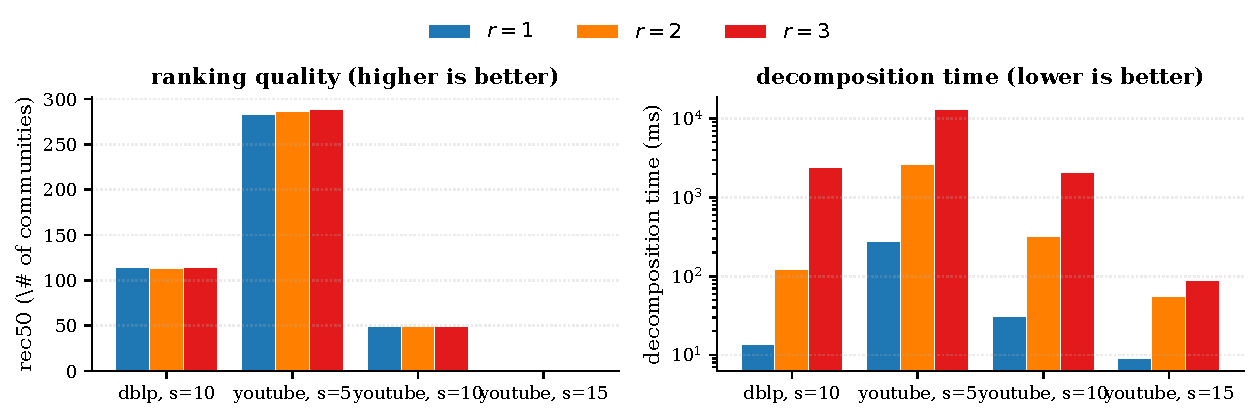
\includegraphics[width=\linewidth]{figures/fig_crossr.pdf}
\caption{Cross-$r$ comparison on \texttt{com-dblp} ($s{=}10$) and \texttt{com-youtube} ($s\in\{5,10,15\}$). Left: ranking quality (rec50, higher is better) is nearly identical across $r$. Right: decomposition time (log scale, lower is better) is $1$--$3$ orders of magnitude smaller at $r{=}1$.}
\Description{Two side-by-side bar charts. Left panel shows rec50 bars within each cell are nearly equal across r=1, 2, 3. Right panel shows decomposition time on a log scale where r=1 bars are dramatically shorter than r=2 and r=3 bars in every cell, with the gap reaching about 178 times on dblp s=10.}
\label{fig:crossr}
\end{figure}

\stitle{Case study 4: identifying ego network on DBLP.}\label{sec:cs-viz}
We build a fresh coauthor graph from the official DBLP XML dump (April 2024 snapshot, $3.4$M authors and $23.0$M coauthorship edges), anchor on Jiawei Han (DBLP key \texttt{Jiawei Han 0001}), and take his $1$-hop coauthor ego ($1{,}358$ vertices).
%
Following NuclearCD's case study II~\cite{NuclearCD}, we compare $s\!=\!3$ vs.\ $s\!=\!10$ under $r\!=\!1$.
%
A vertex is \emph{alive} at $s$ iff it participates in at least one $(1,s)$-nucleus (i.e., $k_{1,s}(v)\!\ge\!1$).
%
At $r\!=\!1$ the alive subgraph is naturally one giant connected component (every coauthor of Han is reachable through some shared collaborator), so we partition it into disjoint dense \emph{modules} via greedy near-clique extraction (size $\ge\!10$, internal edge density $\ge\!0.85$); these modules play the role of NuclearCD CS-II's ``nucleus components''.
%
For each module $C$ let $m_{\mathrm{in}}$ be the internal edges and $m_{\mathrm{cut}}$ the edges from $C$ to other alive vertices.
%
We report conductance $\phi(C)\!=\!m_{\mathrm{cut}}/(2m_{\mathrm{in}}\!+\!m_{\mathrm{cut}})$ and separability $m_{\mathrm{in}}/m_{\mathrm{cut}}$; lower $\phi(C)$ and higher $m_{\mathrm{in}}/m_{\mathrm{cut}}$ indicate better separation.
%
A paper is \emph{collaborative} for $C$ if it contains $\ge\!3$ authors from $C$, and the \emph{active ratio} is the fraction of members appearing in at least one collaborative paper.
%
Figure~\ref{fig:cs9} colours each vertex by its module (top-$K$ largest distinct colours per panel, others gray); Table~\ref{tab:cs9-quality} reports the per-$s$ statistics.

\sstitle{Larger $s$ yields compact and better-separated modules.}
Increasing $s$ from $3$ to $10$ shrinks the alive subgraph from $1{,}293$ to $301$ vertices and reduces the module count from $14$ to $3$.
%
The intra-module edge fraction (edges inside any module / total edges in the alive subgraph) holds steady at $0.40$--$0.41$, but the size-weighted average separability nearly doubles ($1.55\!\to\!2.78$) and the size-weighted average conductance more than halves ($0.368\!\to\!0.163$).
%
So the modules that survive at $s\!=\!10$ stand more sharply against the rest of the ego than the larger and looser modules at $s\!=\!3$.

\sstitle{Larger $s$ preserves the strong-collaboration property.}
Within-module collaboration is uniformly strong at every $s$ we test: the top-$5$ modules at $s\!=\!3$ have an average active ratio of $100\%$, and the three surviving modules at $s\!=\!10$ are also $100\%$ active.
%
The high-$s$ filter therefore retains, not discards, the strong-collaboration property of low $s$: every member of every surviving module appears on a paper with $\ge\!2$ other within-module co-authors.
%
The discriminator between low and high $s$ is structural separation (separability and conductance), not semantic correctness --- high-$s$ modules are real, but they are also \emph{tighter and more cleanly isolated} working groups within Han's collaboration neighbourhood.

\begin{table}[t]
\centering
\caption{Per-$s$ module quality on Han's $1$-hop coauthor ego (Figure~\ref{fig:cs9}). ``Alive'' = vertices in at least one $(1,s)$-nucleus. ``Modules'' = greedy dense partition (size $\ge\!10$, density $\ge\!0.85$). $m_{\mathrm{in}}/m_{\mathrm{cut}}$ and $\phi$ are size-weighted averages over all modules. Active = top-$K$ avg fraction of members in $\ge\!3$-within-module-co-author papers.}
\label{tab:cs9-quality}
\small
\begin{tabular}{rrrcccc}
\toprule
$s$ & alive & \#mods & intra-frac & $m_{\mathrm{in}}/m_{\mathrm{cut}}$ & $\phi$ & top-$K$ active \\
\midrule
 3 & 1293 & 14 & 0.40 & 1.55 & 0.37 & 1.00 (K=5) \\
10 &  301 &  3 & 0.41 & \textbf{2.78} & \textbf{0.16} & 1.00 (K=3) \\
\bottomrule
\end{tabular}
\end{table}

\begin{figure*}[t]
\centering
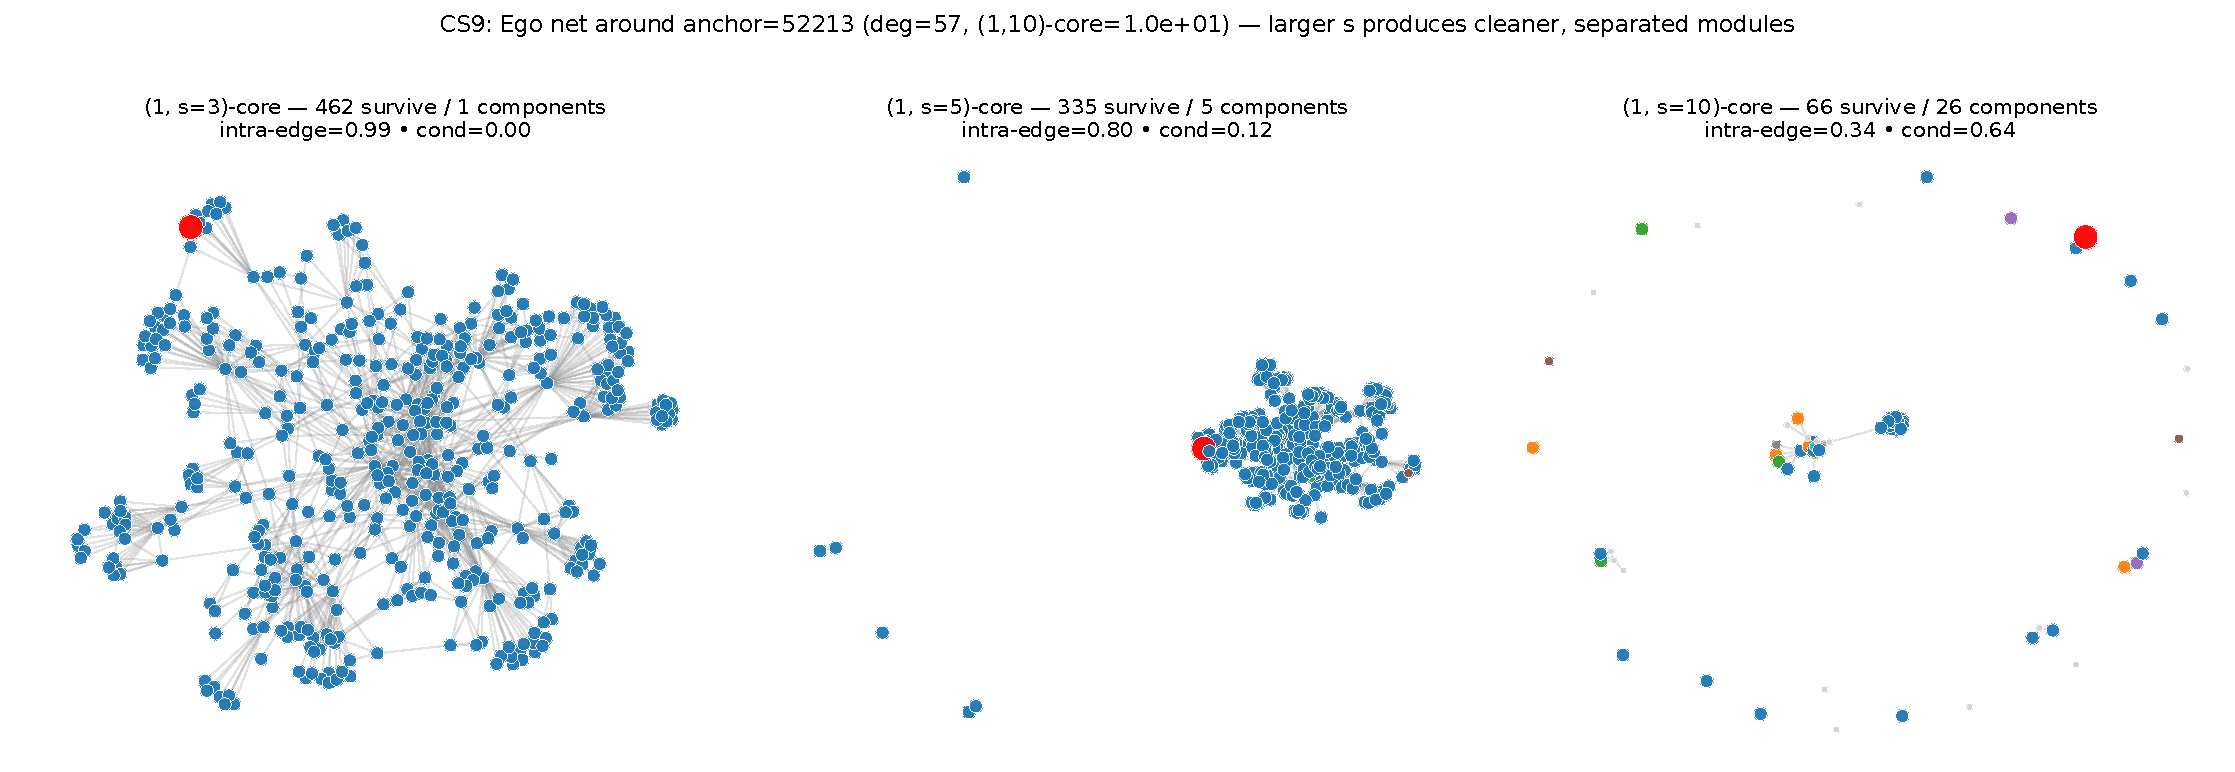
\includegraphics[width=0.95\linewidth]{figures/cs9_egonet.pdf}
\caption{Han's $1$-hop coauthor ego ($1{,}358$ vertices, anchor Jiawei Han $0001$ in red) under $s\!=\!3$ (left) vs.\ $s\!=\!10$ (right) on a shared spring layout. Vertices coloured by their dense module (top-$5$ at $s\!=\!3$, top-$3$ at $s\!=\!10$, each labelled with a representative research focus inferred from the dominant non-CoRR venue of its $\ge\!3$-co-author papers); peeled vertices in light gray, alive-but-not-in-top-$K$ in dark gray. Increasing $s$ consolidates $14$ modules into $3$, nearly doubles the size-weighted average separability ($m_{\mathrm{in}}/m_{\mathrm{cut}}:1.55\!\to\!2.78$), and more than halves the average conductance ($\phi:0.37\!\to\!0.16$); every annotated module is $100\%$ active (every member appears on a paper with $\ge\!3$ within-module co-authors). See Table~\ref{tab:cs9-quality}.}
\Description{Two side-by-side ego-network panels showing Han's 1-hop coauthor neighbourhood at s=3 and s=10. At s=3, five large colored clusters (Data Mining, IR/Web, AI/ML, Multimodal NLP, NLP) spread across the spring layout, each labeled with a callout box giving its member count and paper count. At s=10, three smaller and more isolated colored clusters (ML Safety, Multimodal Web, NLP) remain, while the rest of the ego has been peeled away into light gray.}
\label{fig:cs9}
\end{figure*}

\stitle{Case study 5: hierarchy profiles differ by domain.}\label{sec:cs-hier}
\buildHier{} turns the core values into a $(1,s)$-clique-connected nucleus hierarchy (Definition~\ref{def:nucleus}).
%
This makes it possible to compare how quickly the nucleus hierarchy collapses across domains.
%
Table~\ref{tab:cs10cross} reports the three hierarchy statistics used here.
%
Figure~\ref{fig:cs10} visualizes the resulting join trees side by side.

\begin{table}[t]
\centering
\caption{Nucleus hierarchy summary: number of leaf branches and maximum tree depth at each $s$.}
\label{tab:cs10cross}
\tiny
\setlength{\tabcolsep}{4pt}
\begin{tabular}{@{}l rr rr rr rr@{}}
\toprule
& \multicolumn{2}{c}{$s=3$} & \multicolumn{2}{c}{$s=5$} & \multicolumn{2}{c}{$s=10$} & \multicolumn{2}{c}{$s=15$} \\
\cmidrule(lr){2-3}\cmidrule(lr){4-5}\cmidrule(lr){6-7}\cmidrule(lr){8-9}
graph & \#branches & depth & \#branches & depth & \#branches & depth & \#branches & depth \\
\midrule
\texttt{com-dblp}     & $10{,}900$ & $4$ & $6{,}050$ & $4$ & $751$ & $4$ & $197$ & $4$ \\
\texttt{com-youtube}  & $13{,}507$ & $4$ & $714$ & $3$ & $12$ & $2$ & $1$ & $1$ \\
\texttt{web-Stanford} & $3{,}455$ & $5$ & $1{,}093$ & $3$ & $228$ & $3$ & $90$ & $2$ \\
\bottomrule
\end{tabular}
\end{table}

\texttt{com-youtube} collapses quickly: from $13{,}507$ branches at $s=3$ to a single branch at $s=15$.
%
\texttt{com-dblp} keeps the largest branch counts and a constant maximum depth across $s$, reflecting strong nested clique structure.
%
\texttt{web-Stanford} retains nontrivial branches at every clique size, including $s=15$.
%
Figure~\ref{fig:cs10} makes the contrast visual at $s=5$ by plotting branch persistence ($k_{\mathrm{birth}}-k_{\mathrm{death}}$) against the rank of each branch when sorted by persistence (log--log).
%
\texttt{com-dblp}'s curve is a long flat tail: hundreds of branches retain persistence above $10^2$ and thousands above $10^1$, which is characteristic of a deeply nested hierarchy.
%
\texttt{com-youtube}'s curve drops sharply after the first few ranks and plateaus near persistence $1$, showing that only a handful of branches carry real depth.
%
\texttt{web-Stanford} lies between the two.
%
The hierarchy is therefore not only an output format.
%
It gives a domain-level profile of clique-witness nesting.

\begin{figure}[t]
\centering
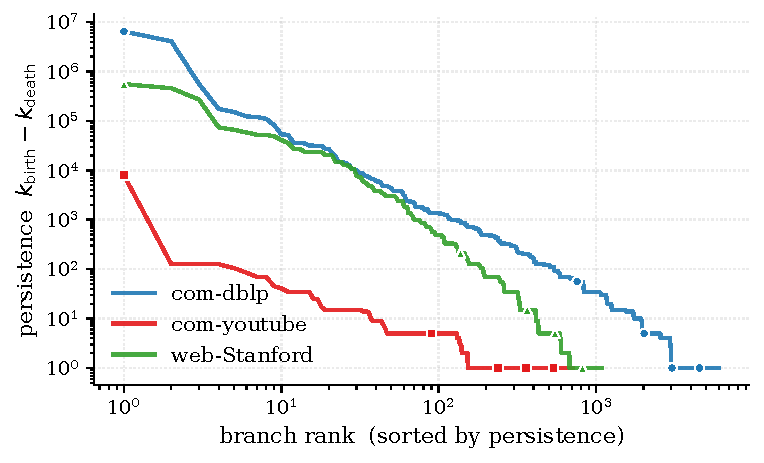
\includegraphics[width=\linewidth]{figures/cs10_hierarchy.pdf}
\caption{Branch persistence vs.\ rank at $s{=}5$ (log--log).}
\Description{Single panel with three log-log curves: com-dblp's persistence stays high for thousands of branches; com-youtube drops sharply after a handful; web-Stanford lies between them.}
\label{fig:cs10}
\end{figure}

\stitle{Takeaway.}\label{sec:cs-summary}
On the DBLP and YouTube community-ranking tasks, $r=1$ matches higher-$r$ quality metrics at much lower cost; the hierarchy and ego-network studies show the same decomposition also yields interpretable local structure and a per-domain hierarchy profile.
%
The evidence is scoped to these datasets and metrics rather than a universal claim, but it is enough to justify optimising the exact $r=1$ case.
